\chapter{Implementation}
\label{chapter:methods}

\section{Overview}
TODO : ADD INTRO LATER HERE



\section{Business Speech (BizSpeech) Dataset}
As mentioned in the Section \ref{section:largescale_related}, there are not many datasets which are available publicly for training speech recognition systems at a scale of around tens of thousands of hours. This section introduces Business Speech dataset, which has been used for all the experiments in this thesis. 

Business speech dataset consists of conference calls, which are corporate disclosure and brokerage event information. It can be accessed through a paid licence here\footnote{Company Events Coverage - StreetEvents - Refinitiv. \href{https://www.refinitiv.com/en/financial-data/company-data/company-events-coverage}{https://www.refinitiv.com/en/ financial-data/company-data/company-events-coverage}}. Refinitiv also provides transcriptions, call summaries and other metadata like date and PermID, which is the ID number for the firm. This ID can further be used to link to many more metadata information from other datasets like the officers and directors dataset\footnote{Officers and Directors data - Refinitiv \href{https://www.refinitiv.com/en/financial-data/company-data/officers-and-director-search}{https://www.refinitiv.com/en/financial-data/ company-data/officers-and-director-search}} which provides information about the firm's financials, personnel involved etc. The audio and transcripts can be accessed via APIs and also via the Eikon software\footnote{Eikon Financial Analysis \& Trading Software - Refinitiv \href{https://www.refinitiv.com/en/products/eikon-trading-software}{https://www.refinitiv.com/ en/products/eikon-trading-software}} \cite{August2011ThomsonEikon}. Figure \ref{fig:eikon} shows a snapshot of the dataset being used.

\begin{figure}[ht]
  \begin{center}
    % below the size of the figure has been reduced for example
    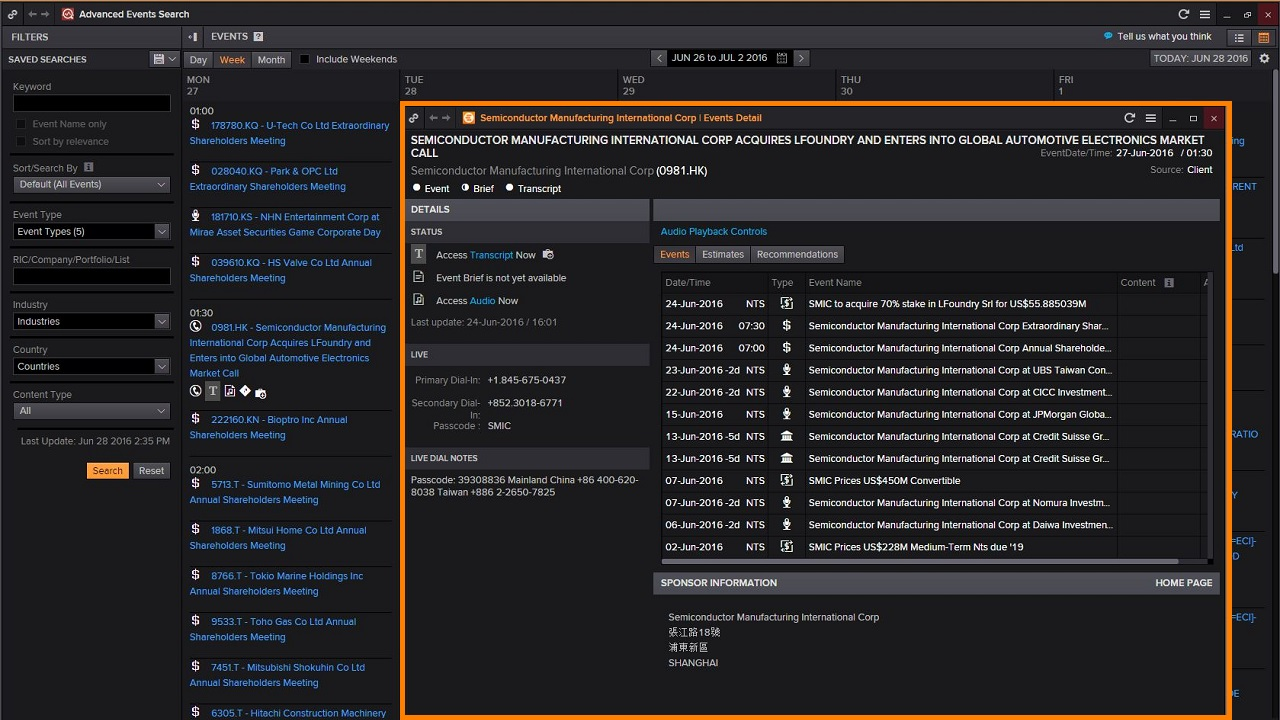
\includegraphics[width=\textwidth]{images/company-events-coverage-eikon.jpg} 
    \caption{Conference call event information in Eikon.}
    \label{fig:eikon}
  \end{center}
\end{figure}

The dataset which is used for the experiments consist of 24,793 conference calls held by 6,131 firms all over the world. All the calls are in English language. Approximately 80\% of the firms are from English-speaking countries. Earnings calls pertaining to fiscal year 2017 contribute to 68\% of the dataset, 22\% are from 2016 and 5\% each is from 2015 and 2018. 
The conference calls are one-hour long conversations with the initial part of the call consists of a presentation about the firm's financials in the previous period and the rest of the call is a question and answer session with journalists and other analysts. Hence, the dataset has different types of speech, prepared one-sided speech is in the first half of the audio and the rest are more conversational in nature. The speech is mostly in the sphere of finance and business and consists of a lot of jargon from this domain. The dataset has different speech from different English accents. An analysis of the companies' metadata show that the dataset consists of conference calls of companies from 76 countries. Out of the 24793 events, 4822 (around 20\%) are from non-native English-speaking countries. Even among the native English-speaking countries, there is a wide distribution of events between the USA, UK, Australia, New Zealand, etc.

Since there are no publicly available results on this dataset for the task of automatic speech recognition, a portion of it was processed using popular cloud speech to text services to analyse the complexity of the dataset. Azure's\footnote{Speech to Text, Audio to Text Translation, Microsoft Azure \href{https://azure.microsoft.com/en-us/services/cognitive-services/speech-to-text/}{https://azure.microsoft .com/en-us/services/cognitive-services/speech-to-text/}} speech to text service and Google's\footnote{Speech-to-Text: Automatic Speech Recognition, Google Cloud \href{https://cloud.google.com/speech-to-text/}{https://cloud.google. com/speech-to-text/}} speech to text services analysed around 2000 randomly sampled utterances from the BizSpeech dataset. The word error rates (WER) on the two services were 19.74\% and 21.9\% on Azure and Google, respectively. Furthermore, on analysing the word error rates based on the nationality of the companies, from Figure \ref{fig:wer_cloud} we can observe that on Google, there is a drop of 49\% in WER and in Azure, the drop is 58\% from native to non-native utterances which shows that even the most generalized models can suffer with different speaking conditions. 

\begin{figure}[ht]
  \begin{center}
    % below the size of the figure has been reduced for example
    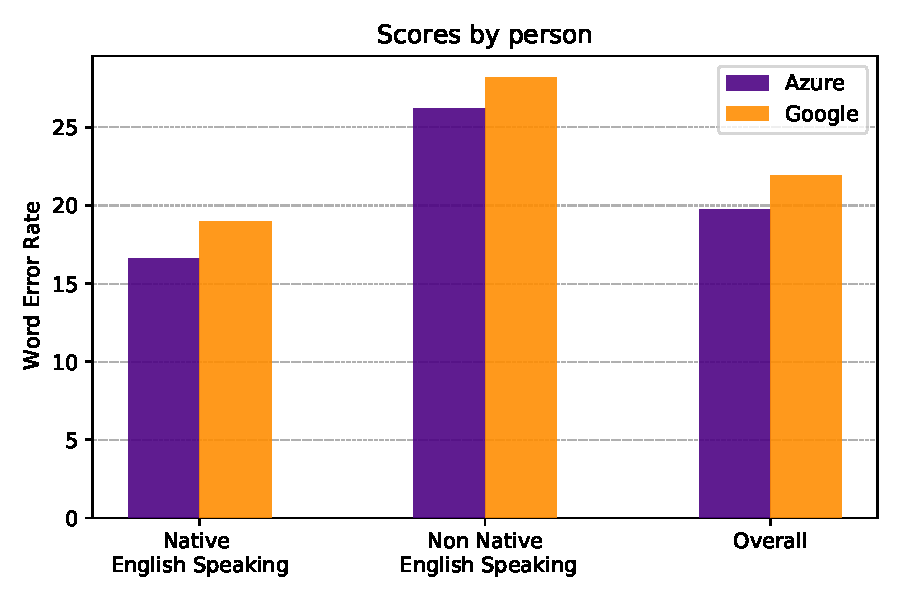
\includegraphics[width=0.8\textwidth]{images/wer_cloud.pdf} 
    \caption{Word Error Rate - Initial Dataset Analysis}
    \label{fig:wer_cloud}
  \end{center}
\end{figure}

 The main advantage of this dataset is that it is quite a large dataset with varies types of speech and with different accents. The drawback of the dataset is that the speech is from a single domain and from a specific field, which might mean that the models trained on this dataset might not be useful for general speech recognition tasks.
 
\section{Data Preparation}
After downloading the dataset, training \acrshort{asr} models still requires a few preprocessing steps. This section explains these preprocessing steps in more detail. 

The audio recordings in the BizSpeech dataset, are a mix of MP3 and WAV files which have varying sampling rates between 8 kHz, 16 kHz and 32 kHz. We convert all the audio to WAV format with 16 kHz sampling rate to maintain uniformity across the whole dataset.

\subsection{Forced Alignment}
Even though they have transcripts for the speech, most of them lack timestamps for the utterances or are inaccurate. The audio files are also around 1 hour long in length, and hence it would be impossible to use the data for training \acrshort{asr} models without finer and accurate timestamps for the sentences. 

\begin{figure}[ht]
  \begin{center}
    % below the size of the figure has been reduced for example
    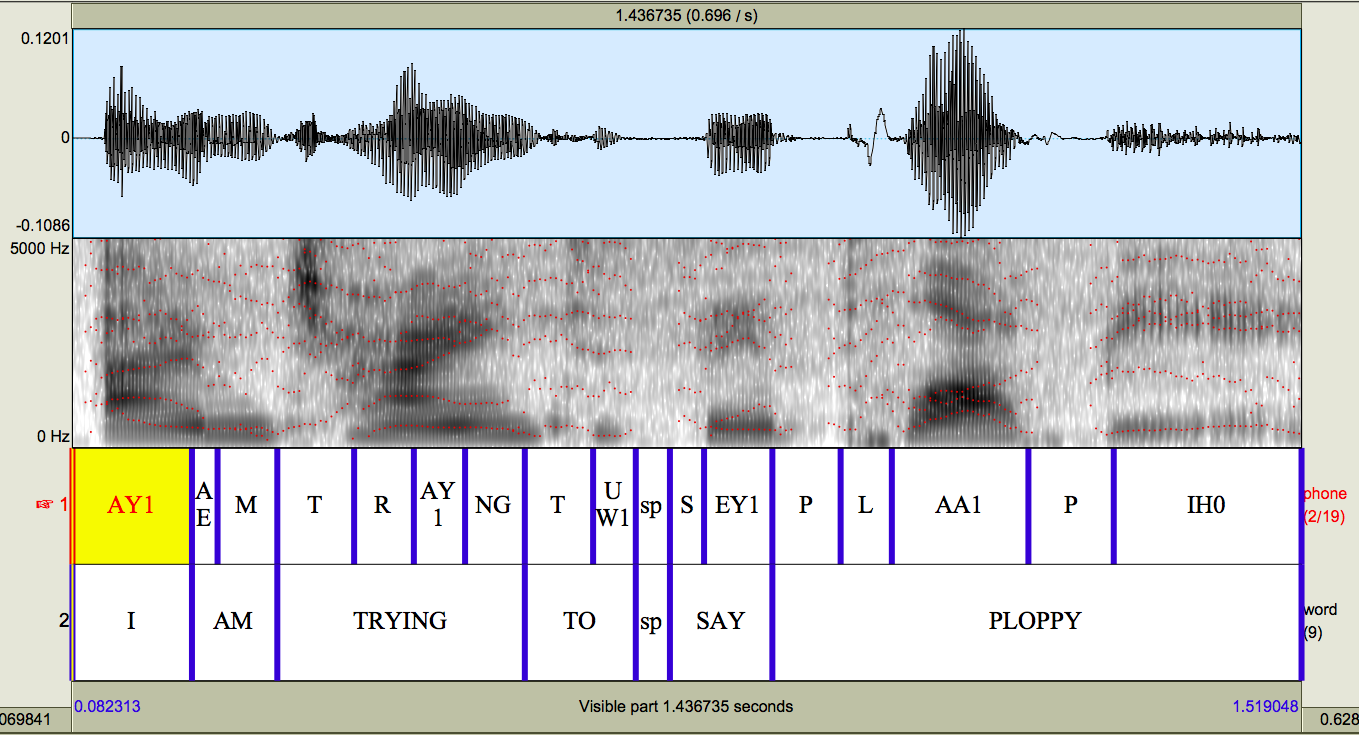
\includegraphics[width=0.8\textwidth]{images/ploppy.png} 
    \caption{Result of forced alignment for an example input. \cite{Yuan2008SPEAKERCORPUS}}
    \label{fig:p2fa}
  \end{center}
\end{figure}

We use forced alignment to generate accurate alignment of speech with the textual data. Forced alignment helps to align linguistic units (e.g., phoneme or words) with the corresponding audio file. It requires an audio file with transcriptions as input, and it outputs the text with word level time-aligned data. We use the P2FA for Python 3\footnote{Penn Phonetics Lab Forced Aligner Toolkit (P2FA) for Python3, \href{https://github.com/jaekookang/p2fa\_py3}{https://github.com/ jaekookang/p2fa\_py3}} tool, which is a \acrshort{hmm} forced aligner based on P2FA \cite{Yuan2008SPEAKERCORPUS} to generate alignments. The aligner works by using a HTK \cite{Young2002TheBook} based acoustic model along with a pronunciation dictionary. The tool generates the transcript's phoneme representation, and then the acoustic model is used to generate accurate time-aligned output. An example of this can be seen in Figure \ref{fig:p2fa}.

As mentioned in their work, the errors for the successful alignments are around 50ms. A risk of using forced aligner is that it always tries to generate some sort of alignment. When any sorts of inconsistencies are present with the text and audio, for example, a missing word in the transcript, can deceive the tool for the whole file's alignment and the tool fails. It is difficult to automatically detect these cases and a human test is expensive, especially at the scale of the BizSpeech dataset. Due to this issue, \emph{the usable data from the 24,793 audio hours for training \acrshort{asr} model is finally 19973 hours with close to 9 million utterances with a composition of 52,484 speakers.}

\subsection{Data Loading Performance}
Now that accurate time alignments are available for the dataset, the large audio files are split into smaller files such that each audio split has one sentence in it. Each one of these sentence is used as an utterance and is stored as a WAV file. The text for the audio file is stored in a JSON file along with a few metadata fields, with a unique utterance ID as the filename for both the audio clip and the JSON file. 


Each utterance length ranges from one second up to 60 seconds. Figure \ref{fig:utt_dist} shows the distribution of the utterance length for the whole dataset. We can see that most of the utterances are around the 6-second length. Since, the utterances are small in relative to the overall size of the dataset (close to 20,000 hours) there are about 9 million audio files and 9 million JSON files to be loaded for every training run. This becomes highly inefficient and will usually lead to problems opening too many files on the training node. The size of the dataset is also around 5 TB, which makes it hard to store on a single disk storage. All these problems lead to extremely high usage of disk storage, disk I/O usage, network costs (especially for multi node training), and high CPU usage to access and read a high number of files. 


\begin{figure}[ht]
  \begin{center}
    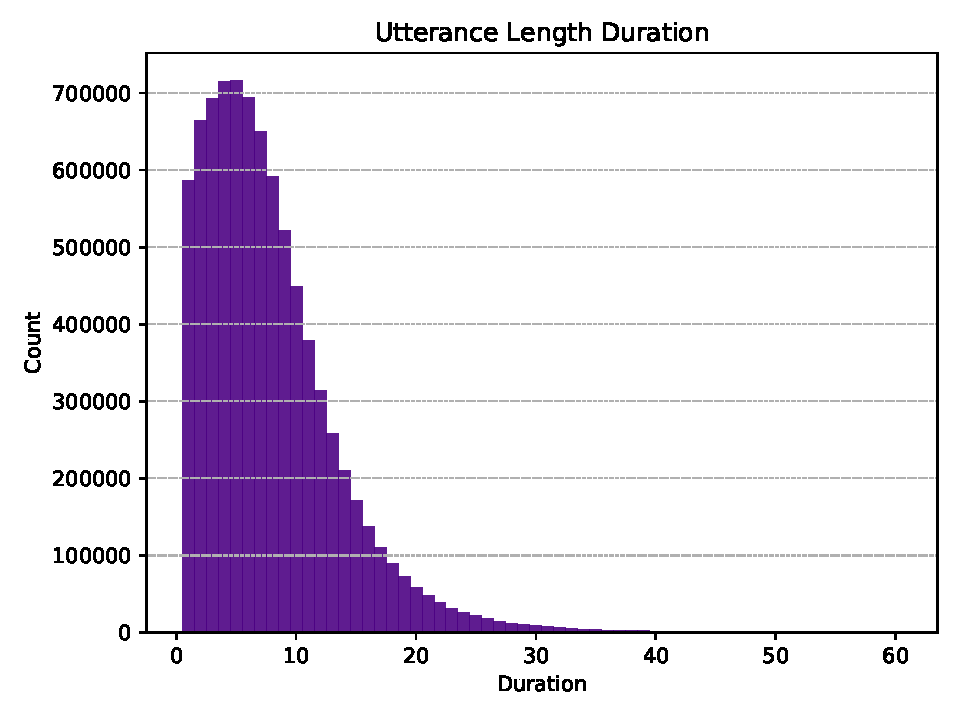
\includegraphics[width=\textwidth]{images/duration_distribution.pdf} 
    \caption{Utterance Duration Distribution for BizSpeech Dataset}
    \label{fig:utt_dist}
  \end{center}
\end{figure}

Hence, we use WebDataset\footnote{webdataset/webdataset: A high-performance Python based I/O system for large (and small) deep learning problems, with strong support for PyTorch. \href{https://github.com/webdataset/webdataset/}{https://github.com/ webdataset/webdataset/}}\cite{Aizman2019HighLearning}, a PyTorch Dataset (\inlinecode{IterableDataset}\footnote{torch.utils.data, PyTorch 1.9.0 documentation \href{https://pytorch.org/docs/stable/data.html}{https://pytorch.org/docs/stable/data .html}}) implementation which provides high efficiency access to data stored in TAR\footnote{GNU tar 1.34: Basic Tar Format \href{https://www.gnu.org/software/tar/manual/html_node/Standard.html}{https://www.gnu.org/software/tar/manual/html\_ node/Standard.html}} archives. This uses only sequential/streaming data access, which brings substantial performance advantage. Figure \ref{fig:seq} shows, on the left side, a file-based access to resources and on the right side, an illustration of sequential based access to resources. We can see from the illustration that sequential data access is much faster and requires much lesser communication. Typically, a ten-fold increase in performance can be seen during I/O operations\cite{Aizman2019HighLearning} for a single node setup with sequential access. This enables large-scale training. Because, it supports basic TAR archives the other advantage is that it becomes easy to create, manage and distribute the data for deep learning training. Since, TAR can be compressed using gzip\footnote{gzip, Wikipedia \href{https://en.wikipedia.org/wiki/Gzip}{https://en.wikipedia.org/wiki/Gzip}} and this is supported directly by webdataset and this helps to save storage space as well. Webdataset can also be set up to use sharding. Sharding helps achieve high throughput using parallel I/O with multiprocess enabled tasks like data loading, preprocessing, etc. This. We specify the shards as a list of files to webdataset, or they can be written using the brace notation. For example, \inlinecode{bizspeech-shard-\{000000..003000\}.tar} means there are 3000 shards. When used with a standard Torch \inlinecode{DataLoader}, this will perform parallel I/O and preprocessing. 


\begin{figure}[ht]
  \begin{center}
    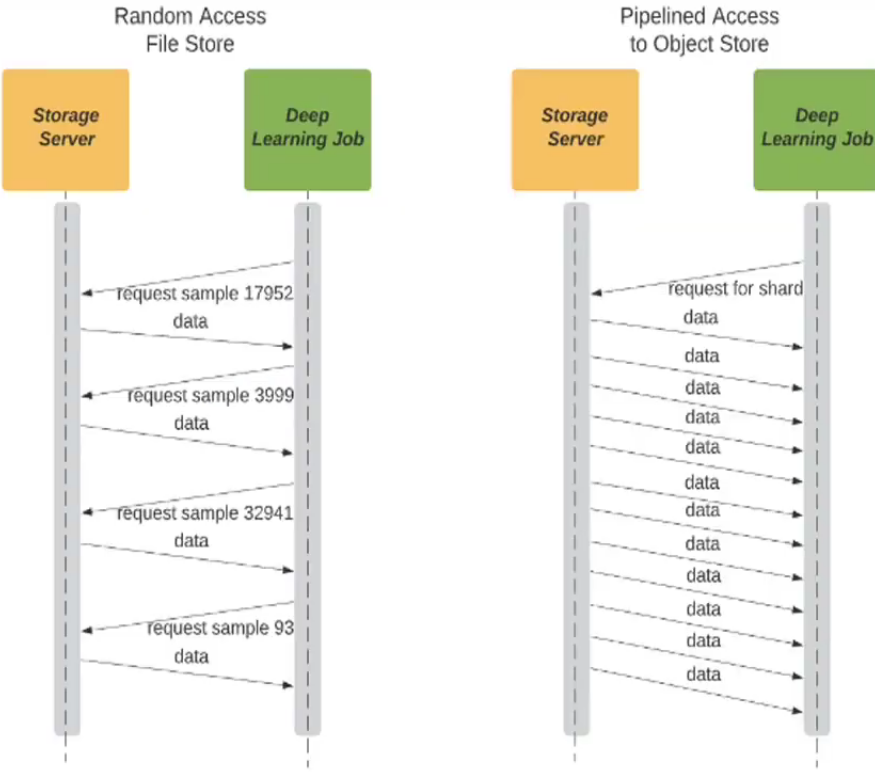
\includegraphics[width=0.7\textwidth]{images/sequential.png} 
    \caption{File-based Access vs Sequential Data Access \cite{Aizman2019HighLearning}}
    \label{fig:seq}
  \end{center}
\end{figure}

\emph{We convert the BizSpeech dataset  to compressed tar to enable usage of webdataset. Split the dataset into 3000 shards, with each shard containing about 700 MB of data after compression, totalling at around 2.1 TB storage footprint. This dataset is now ready to be used for training ASR models efficiently. Empirically, speed-up after using webdataset with a single process was around 7-8 fold during training a small subset of 80 hours of the dataset. It becomes very difficult practically to store and test the file-based mechanism to measure the throughput difference for very large-scale experiments. For all the large-scale experiments of order more than 200 hours, we use a configuration of 2-4 worker processes per GPU with sharding and randomization enabled.}

\section{Training Attention based Encoder-Decoder model}
For training a speech to text model on BizSpeech dataset, we use SpeechBrain (introduced in Section \ref{section:sb}). SpeechBrain provides recipes which are designed and further optimized for particular datasets. Considering the scale of experiments, we use the LibriSpeech recipe\footnote{speechbrain/recipes/LibriSpeech/ASR/seq2seq \href{https://github.com/speechbrain/speechbrain/tree/develop/recipes/LibriSpeech/ASR/seq2seq}{https://github.com/speechbrain/spee chbrain/tree/develop/recipes/LibriSpeech/ASR/seq2seq}} as a starting point for our experiments. After data loading and basic preprocessing to parse the audio and transcript text, we generate features from the audio signal. We use logarithmic, Mel-based, Filter Banks with  0-8000 Hz frequency and the processing happens on-the-fly with data loading. These steps can be parallelized easily by enabling multiprocessing to increase the number of available workers loading the data. From the recipe, we disable the Language Model for our experiments because the focus is on scaling up the training of speech to text and not necessarily to make the model the most accurate one. The final model and configuration used is given in the Appendix \ref{chapter:model-architecture}. We use the negative log likelihood loss function along with the CTC loss (described in Section \ref{section:ctc}) for the initial 15 epochs. 

\subsection{Dynamic Batching}
A problem in automatic speech recognition is when batching up the utterances for training, the varying lengths of utterances means that the shorter utterances have to be padded up to the length of the longest utterance in the batch. Depending on the ordering of the utterances, the batches of data used for training could be high in sparsity due to padding. Because the ordering of training data is usually random, a fixed batch size can be inefficient when the utterances are short. To counter this, we sort the speech data in length to make the \acrshort{gpu} usage more efficient. However, this may affect the model convergence based on the type of ordering used. To solve these problems, SpeechBrain has a dynamic batching data loader, which is 
\subsection{Evaluation Criteria}

\section{Multi-GPU training}
\subsection{Synchronous Training-DDP}
\subsection{Asynchronous Training-HOGWILD!}